% Vorlage fuer latex-beamer-Praesentationen unter Verwendung des Corporate 
% Designs der Uni.
%
% Basiert auf der alten Vorlage von Carsten Bockelmann 
% (bockelmann@ant.uni-bremen.de), angepasst an das Corporate Design von 
% Henning Paul (paul@ant.uni-bremen.de) unter Verwendung der Vorlage von
% Dirk Lorenz und Kristan Bredies aus dem Zentrum fuer Technomathematik
% ({dlorenz,kbredies}@math.uni-bremen.de)

\documentclass[10pt]{beamer}

\mode<presentation>
{
  % Das ANT-Theme benutzen
  % Titel in Kopfzeile, kleine Navigationselemente, Seitennummer anzeigen,
  % Autor dauerhaft eingeblendet lassen
  % \usetheme[headlinetitle,navline=small,footlinenumber,footlineauthor]{ANT}

  % Autor nicht dauerhaft einblenden
   \usetheme[headlinetitle,navline=small,footlinenumber]{Bremen}

  %
  % Die vollstaendige Dokumentation zu unserem Theme findet sich in der Datei 
  % beamerZeTeMdoc.pdf, da es auf dem Theme der Technomathematiker aus dem 
  % ZeTeM basiert.
  %
  % Es koennen bis zu zwei zusaetzliche Logos (zu unserer Ameise oben links
  % und dem Uni-Logo unten links) hinzugefuegt werden, diese erscheinen dann
  % rechts neben dem Uni-Logo.
  % \partnerlogo{
	% \includegraphics[height=2.6\baselineskip]{TZI.pdf}}
  % \secondarypartnerlogo{
	% \includegraphics[height=2.6\baselineskip]{DFG_zweizeilig_blau.pdf}}

  % Dieses sind Standard-latex-beamer-Optionen:
  %
  % Der mathematische Schriftsatz ist mit Serifen
  \usefonttheme[onlymath]{serif}
  % Noch nicht aufgedeckte Punkte erscheinen ausgegraut
  \setbeamercovered{transparent}
  % Bild-/Tabellenueberschriften sind sehr klein
  \setbeamerfont{caption}{size=\tiny}

}



%\usepackage[german]{babel}
% oder was auch immer

\usepackage[utf8]{inputenc}
% oder was auch immer

\usepackage{color,soul}
\definecolor{darkblue}{rgb}{0,0,0.5}
\setulcolor{darkblue}

\usepackage{hyperref}
\hypersetup{
    pdftitle={},
    pdfsubject={},
    pdfauthor={Sadik Özoguz},
    pdfkeywords={},
    % pdfpagemode=None, %deprecated
    plainpages=false,
    pdfstartview=Fit,
    breaklinks=true,
    colorlinks=false,
    pdfhighlight=/N,
    % define colors, even if not used
    linkcolor=blue,
    citecolor=blue,
    urlcolor=blue,
    citebordercolor=1 1 1,
    filebordercolor=1 1 1,
    linkbordercolor=1 1 1,
    menubordercolor=1 1 1,
    % pagebordercolor=1 1 1, %deprecated
    urlbordercolor=1 1 1,
    % pdfborder=1 1 1 %erzeugt fehler im footer
  }

\title{Eigenschaftsorientiertes Testen sicherheitskritischer Systeme}
\author{Sadik Özoguz}
\institute{Universit{\"a}t Bremen}
\date[02.02.2018]{2. Februar 2018}

\newcommand{\W}{\mathcal{W}}
\newcommand{\F}{\mathcal{F}}

\subject{Presentation}
\AtBeginSection[]
{
  \begin{frame}
    \frametitle{Überblick}
    \tableofcontents[currentsection]
  \end{frame}
}

% Hier beginnt der redaktionelle Inhalt

\usepackage[ngerman]{babel}
\addto{\captionsngerman}{%
  \renewcommand*{\contentsname}{Inhalt}
  \renewcommand*{\listfigurename}{Abbildungen}
  \renewcommand*{\listtablename}{Tabellen}
  \renewcommand*{\figurename}{Abb.}
  \renewcommand*{\tablename}{Tab.}
}

\begin{document}

\begin{frame}
  \titlepage
\end{frame}

\section*{Überblick}
\begin{frame}<beamer>
  \frametitle{Überblick}
  \tableofcontents
\end{frame}

\section{Einleitung / Motivation}

\begin{frame}
  \frametitle{Motivation}
  \begin{itemize}
    \item MBT: Modell $\rightarrow$ (vollständige) Test Suite
    \item Je größer die Test Suite, desto teurer das Testen
    \item<2-> Stattdessen: Nachweis einer Eigenschaft
    \item<3-> Ziel: Kleinere Testsuite, aber vollständig bezüglich dieser Eigenschaft
  \end{itemize}
\end{frame}

\section{DFSM}
\subsection{Definition}
\begin{frame}
  \frametitle{DFSM}

  \begin{definition}[Deterministische Finite State Machine]
    Eine deterministische Finite State Machine (DFSM) ist ein 5-Tupel $$M=(Q,q_0,\Sigma_I,\Sigma_O,h)$$
    $Q$: Zustandsraum\\
    $\Sigma_I$, $\Sigma_O$ : Ein-, Ausgabealphabet\\
    $h \subseteq Q \times \Sigma_I \times \Sigma_O \times Q$ : Übergangsrelation 
  \end{definition}
  Deterministisch: $(q,x,y_1,q_1),(q,x,y_2,q_2) \in h: (y_1 = y_2 \wedge q_1 = q_2)$
\end{frame}

\subsection{Eigenschaften}
\begin{frame}
\frametitle{FSM Eigenschaften}
\begin{itemize}
  \item<1-> Vollständig (\emph{input complete})$$\forall q\in Q, x\in \Sigma_I : \exists y \in \Sigma_O, q'\in Q : (q,x,y,q')\in h$$
  \item<2-> Die Sprache eines Zustandes $q \in Q$ ist eine Menge von Eingabe-/Aus\-gabefolgen $$L(q)= \{\overline{x}/\overline{y}\ | \exists q' \in Q : (q,\overline{x}, \overline{y}, q') \in h \}$$
  \item<3-> I/O-äquivalent: $L(q_1) = L(q_2)$ bzw. $L(M_1) = L(M_2)$ $$q_1 \sim q_2, M_1 \sim M_2$$
  \item<4-> Minimal: Wenn keine zwei Zustände einer DFSM zueinander äquivalent sind, ist die DFSM \emph{minimal}.
\end{itemize}
\end{frame}
\section{Vollständige Test Suites}
\subsection{$\W$-Methode}
\begin{frame}
  \frametitle{$\W$-Methode}
  \begin{definition}[$\W$-Methode]
  Gegeben ist eine vollständige, minimale DFSM $M$ mit $n$ Zuständen, dann definiert die $\W$-Methode eine $m-$vollständige Testsuite T für $M$ mit
  $$T_\W(M) = V.\bigcup\limits_{i=0}^{m-n+1}\Sigma_I^i.W$$
  bzgl. der Fault Model $\F(M, \sim, \texttt{Dom})$.
  \end{definition}
  \pause
  \begin{itemize}
    \item<2-> $V$ : State Cover
    \item<3-> $W$ : Characterization Set
    \item<4-> $m \in \mathbb{N}$ mit $m \geq n$ (max. Zustände in der Implementierung)
    \item<5-> $\texttt{Dom} = DFSM_C(\Sigma_I, \Sigma_O, m)$ 
  \end{itemize}

\end{frame}

\subsection{$\W_p$-Methode}
\begin{frame}
  \frametitle{$\W_p$-Methode}
  \begin{definition}[$\W_p$-Methode]
  Gegeben ist eine vollständige, minimale DFSM $M$ mit $n$ Zuständen, dann definiert die $\W_p$-Methode eine $m-$vollständige Testsuite T für $M$ mit
  $$T_{\W_p}(M) = (V.\bigcup\limits_{i=0}^{m-n}\Sigma_I^i.W) \cup (V.\Sigma_I^{m-n+1} \oplus {W_q}) $$
  bzgl. der Fault Model $\F(M, \sim, \texttt{Dom})$.
  \end{definition}
  \begin{itemize}
    \item $V$ : State Cover
    \item $W$ : Characterization Set
    \item $\{W_q\}$ : State Identification Sets
    \item $m \in \mathbb{N}$ mit $m \geq n$ (max. Zustände in der Implementierung)
    \item $\texttt{Dom} = DFSM_C(\Sigma_I, \Sigma_O, m)$ 
  \end{itemize}

\end{frame}


\subsection{$H$-Methode}
\begin{frame}
  \frametitle{Vergleich von Methoden}
  \begin{figure}
	  \caption{Quelle: \emph{A. T. Endo and A. Simao, "Experimental Comparison of Test Case Generation Methods for Finite State Machines," 2012 IEEE Fifth International Conference on Software Testing, Verification and Validation, Montreal, QC, 2012, pp. 549-558.} }
	  \centering
	  \includegraphics[width=0.85\textwidth]{images/methodComparison}
	\end{figure}

\end{frame}

\begin{frame}
  \frametitle{$H$-Methode}
  DFSM sei vollständig und minimal
  \begin{itemize}
    \item $A=V\times V$
  	\item $B=V\times (V.\bigcup\limits_{i=1}^{m-n+1}.\Sigma_I^i)$
  	\item $C=\{(\alpha,\beta)|\alpha,\beta\in V.\bigcup\limits_{i=1}^{m-n+1}.\Sigma_I^i, \alpha \in \text{Pref}(\beta)\}$
  \end{itemize}
  Für alle Paare $(\alpha, \beta) \in A\cup B \cup C$, falls $\delta(q_0,\alpha) \not \sim \delta(q_0,\beta)$, dann enthält die Test Suite $\alpha.\omega,\beta.\omega$. $\omega$ ist die \emph{distinguishing trace} für $\delta(\alpha)$ und $\delta(\beta)$.
\end{frame}

\begin{frame}
\frametitle{$H$-Methode - Beispiel}
\begin{columns}[T] % align columns

\begin{column}{.4\textwidth}
\textbf{Liste von Paaren $(\alpha,\beta)$}\\
  \begin{itemize}
	\item<1>$V.\bigcup\limits_{i=1}^{m-n+1}.\Sigma_I^i$
	\item<2-3>\only<1-2>{$(aa,b)$}\only<3->{$(aa,b) \rightarrow a$}
    \item<4-5>\only<1-4>{$(aa,\epsilon)$}\only<5->{$(aa,\epsilon) \rightarrow b$}
    \item<6-7>\only<1-6>{$(ba,a)$}\only<7->{$(ba,a) \rightarrow a$}
    \item<8-9>\only<1-8>{$(ba,\epsilon)$}\only<9->{$(ba,\epsilon) \rightarrow a$}
    \item<10-11>\only<1-10>{$(ab,a)$}\only<11->{$(ab,a) \rightarrow a$}
    \item<12-13>\only<1-12>{$(bb,a)$}\only<13->{$(bb,a) \rightarrow b$}
  \end{itemize}
\end{column}%

\begin{column}{.70\textwidth}
\centering
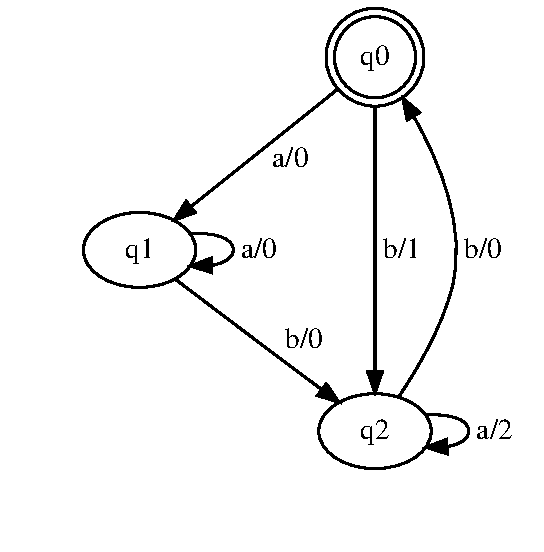
\includegraphics[width=0.5\textwidth]{images/fsm-example01_orig}%
\only<1-2>{\includegraphics[width=0.5\textwidth]{images/HTree01}}%
\only<3>{\includegraphics[width=0.5\textwidth]{images/HTree02_c}}%
\only<4>{\includegraphics[width=0.5\textwidth]{images/HTree02}}%
\only<5>{\includegraphics[height=0.6\textheight]{images/HTree03_c}}%
\only<6>{\includegraphics[height=0.6\textheight]{images/HTree03}}%
\only<7>{\includegraphics[height=0.6\textheight]{images/HTree04_c}}%
\only<8>{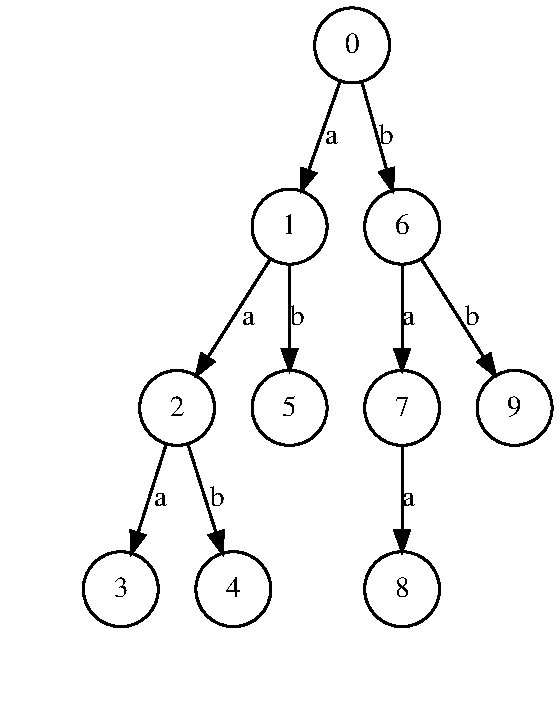
\includegraphics[height=0.6\textheight]{images/HTree04}}%
\only<9>{\includegraphics[height=0.6\textheight]{images/HTree05_c}}%
\only<10>{\includegraphics[height=0.6\textheight]{images/HTree05}}%
\only<11>{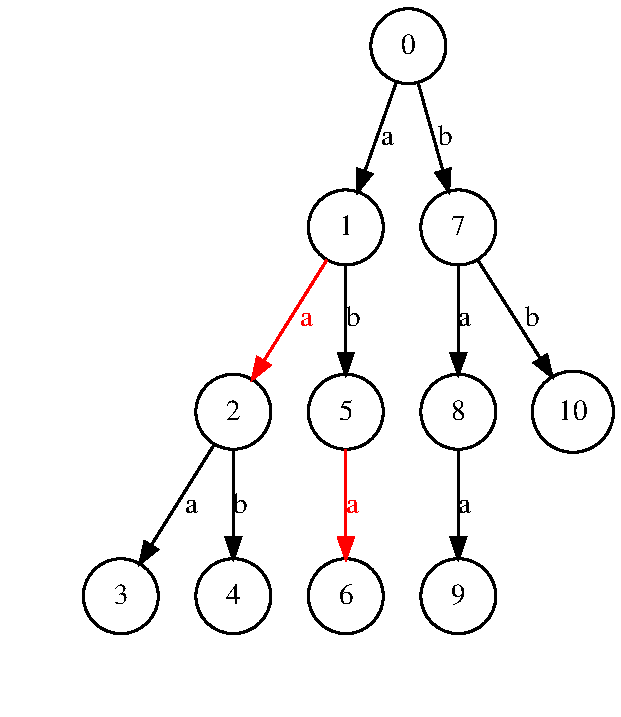
\includegraphics[height=0.6\textheight]{images/HTree06_c}}%
\only<12>{\includegraphics[height=0.6\textheight]{images/HTree06}}%
\only<13>{\includegraphics[height=0.6\textheight]{images/HTree07_c}}%
\only<14>{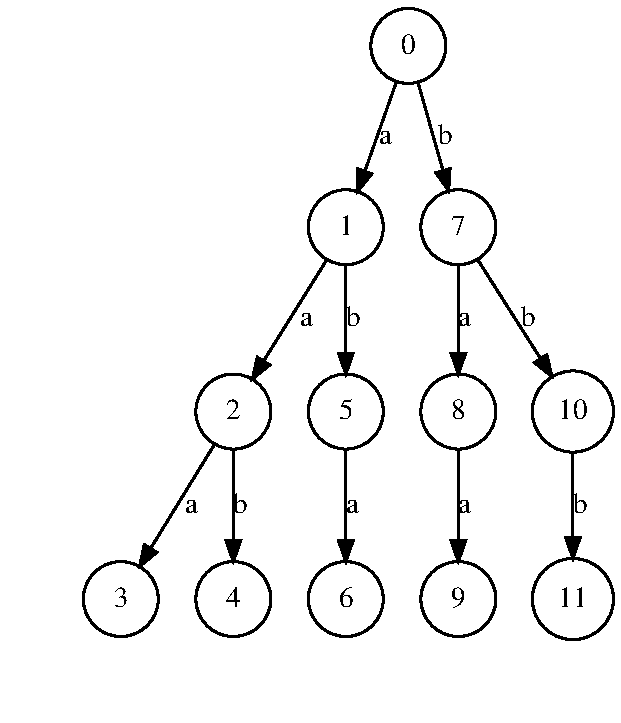
\includegraphics[height=0.6\textheight]{images/HTree07}}%
\end{column}%

\end{columns}
\end{frame}

\begin{frame}
\frametitle{$H$-Methode - Vergleich}
\begin{columns}[T] % align columns

\begin{column}{.7\textwidth}
\begin{itemize}[<+->]
    \item $\W$-Methode: 8 Testfälle, 24 Testschritte
    \item $\W_p$-Methode: 7 Testfälle, 21 Testschritte
    \item $H$-Methode: 5 Testfälle, 15 Testschritte
\end{itemize}
\end{column}%

\begin{column}{.50\textwidth}
\centering
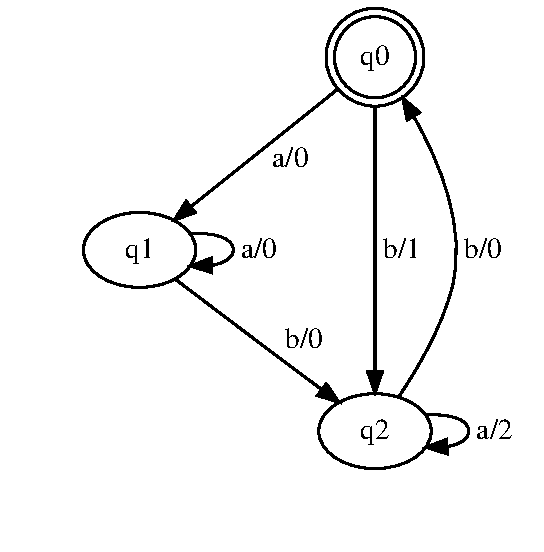
\includegraphics[width=\textwidth]{images/fsm-example01_orig}%
\end{column}%

\end{columns}
\end{frame}

\begin{frame}
\frametitle{$H$-Methode - Optimierung}
Wahl von $\omega$ vom aktuellen Testbaum abhängig machen.

\begin{itemize}
      \item<2-> Ideal: Für $(\alpha, \beta$) finde $\omega$, sodass $\alpha.\omega$ und $\beta.\omega$ im Testbaum
      \item<3-> Sonst: Erweitere bestehenden Test
      \item<4-> Wenn nicht anders möglich: Neuer Testfall 
    \end{itemize}
\end{frame}

\begin{frame}
  \frametitle{$H$-Methode - Optimierung}

  \begin{columns}[T] % align columns
    \begin{column}{.3\textwidth}
	    \begin{itemize}
		  \item Betrachte $(c.a,d)$
		  \item mögliches $\omega: e$
	    \end{itemize}
    \end{column}%

    \begin{column}{.70\textwidth}
        \only<1->{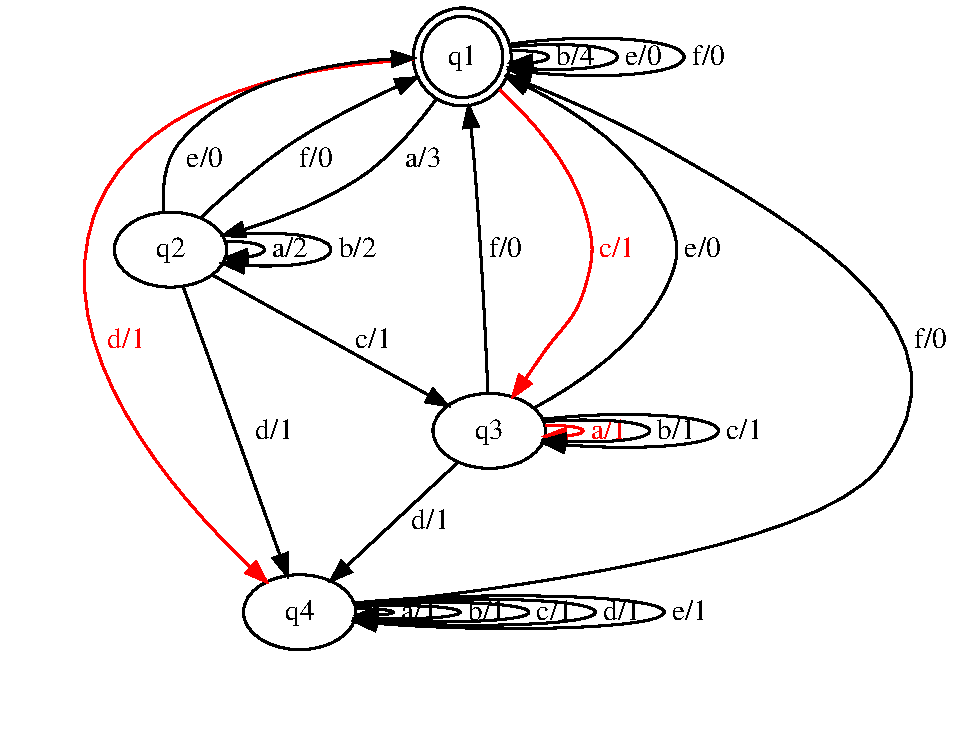
\includegraphics[width=\textwidth]{images/FSM_opt}}
    \end{column}%
  \end{columns}
\end{frame}


\begin{frame}
  \frametitle{$H$-Methode - Optimierung}
  \begin{columns}[T] % align columns

\begin{column}{.4\textwidth}
  \begin{itemize}
	\item<2->Wahl $e$ für $\omega$ würde neuen Test erzeugen
	\item<3->Versuche bestehenden Test zu erweitern
	\item<4->$a.e$ statt $e$
  \end{itemize}
\end{column}%

\begin{column}{.70\textwidth}
Zu diesem Zeitpunkt sieht der Testbaum so aus:
\only<1>{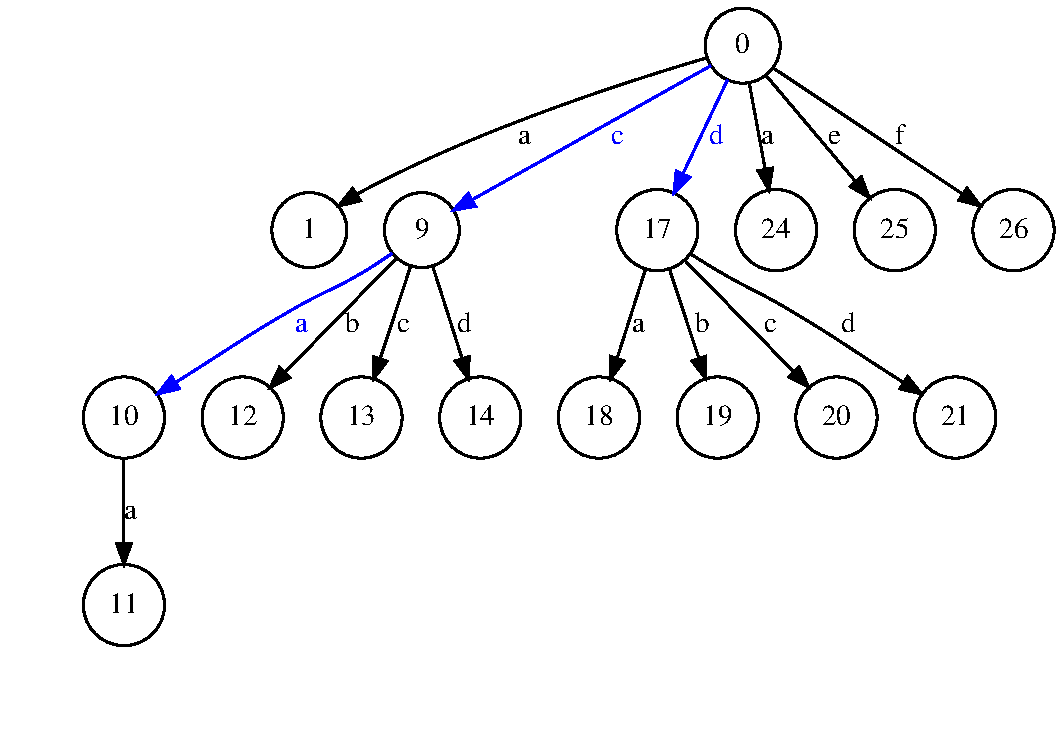
\includegraphics[height=0.6\textheight]{images/HTree_opt}}
\only<2-3>{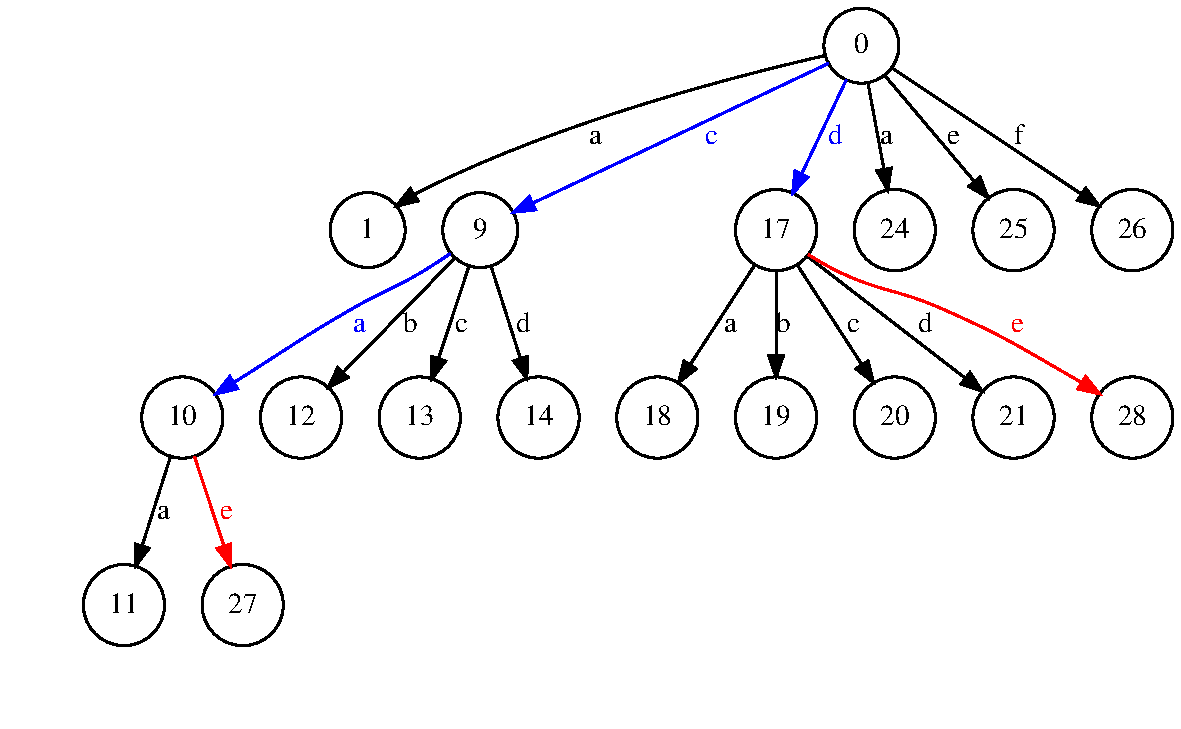
\includegraphics[height=0.6\textheight]{images/HTree_opt2}}
\only<4->{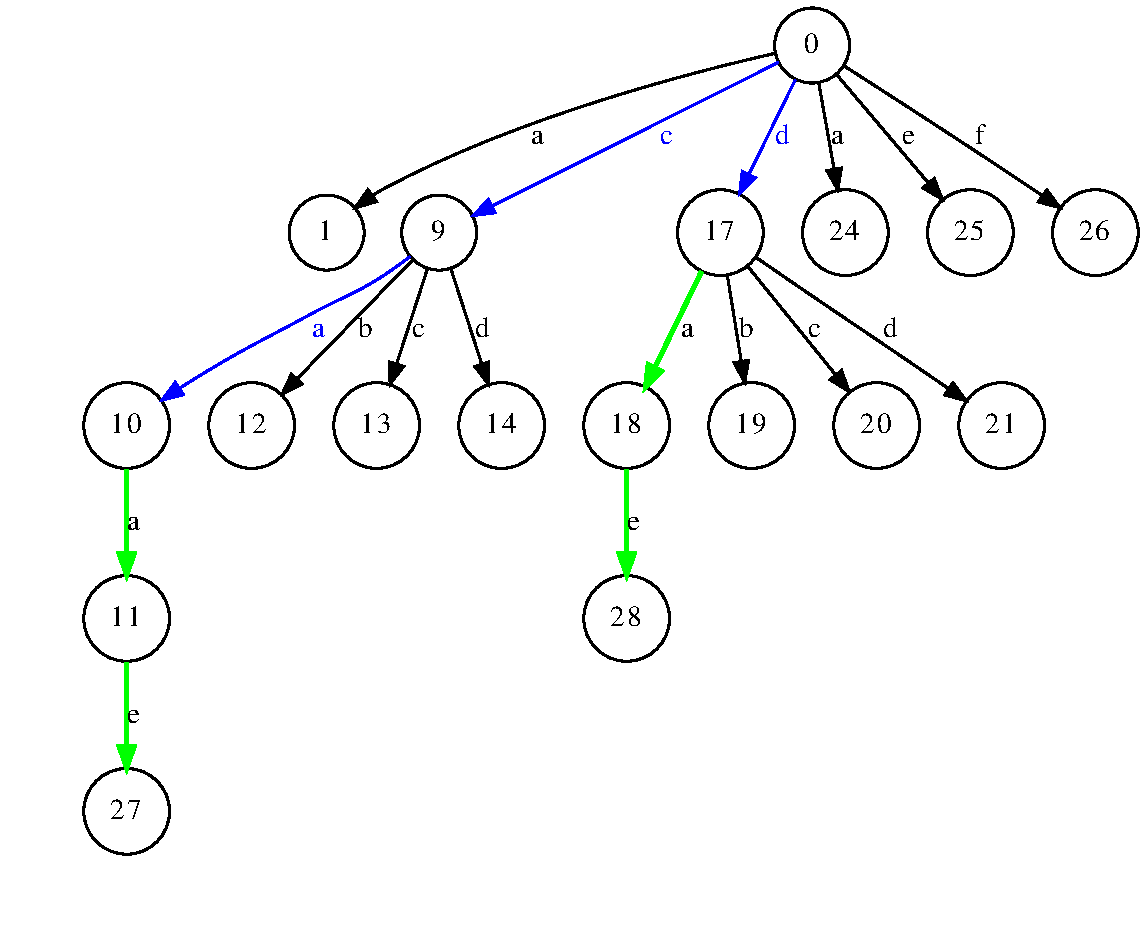
\includegraphics[height=0.7\textheight]{images/HTree_opt3}}
\end{column}%

\end{columns}

\end{frame}

\section{Safety-Vollständigkeit}
\begin{frame}
\frametitle{Safety-related Output Abstraction}
\begin{itemize}
  \item<1-> Reaktion des Systems wird durch DFSM-Ausgabe modelliert
  \item<2-> Idee: Falsche Ausgabe muss nicht sicherheitsrelevant sein
  \item<3-> Sicherheitskritische Reaktionen definieren
  \item<4-> Nicht-sicherheitskritische Reaktionen zusammenfassen
\end{itemize}
\end{frame}

\begin{frame}
\frametitle{safety-Äquivalenz}
\begin{itemize}
  \item<1-> \emph{safety related output abstraction}: $\leq_s \subseteq \Sigma_O \times \Sigma_O$
  \item<2-> $\leq_s$ sei reflexiv, transitiv.
  \item<3-> s-äquivalent: $y_1 \sim_s y_2 \equiv y_1 \leq_s y_2$ und $y_2 \leq_s y_1$
  \item<4-> Zwei I/O-Folgen $X/Y, X'/Y'$ sind s-äquivalent gdw. $X=X'$ und $Y$ und $Y'$ sind s-äquivalent
  \item<5-> Zwei Zustände $q, q'$ sind s-äquivalent gdw. die Outputs für jede Inputfolge s-äquivalent sind.
  \item<6-> Zwei Systeme sind s-äquivalent gdw. ihre Anfangszustände s-äquivalent sind.
\end{itemize}
\end{frame}

\begin{frame}
\frametitle{Safety-Complete Test Suite}
Eine Test Suite $TS$ wird \emph{safety complete} genannt, gdw. für jede IUT $M'$ der Fehlerdomain gilt:
\begin{itemize}
  \item<1-> Soundness: $M$ und $M'$ sind I/O-äquivalent zueinander $\Rightarrow$ $M'$ besteht die Teset Suite ($M'~ \underline{pass}~ TS$)
  \item<2-> safety-Exhaustiveness: Für alle $M'$ aus der Fehlerdomain gilt: $M' \not \sim_s M \Rightarrow M'~ \underline{fail}~ TS$
\end{itemize}
\end{frame}

\begin{frame}
\frametitle{Beispiel}
\begin{columns}[T] % align columns

\begin{column}{.50\textwidth}
\textbf{M}
\includegraphics[width=\textwidth]{images/fsm-example01}
\end{column}%

\begin{column}{.50\textwidth}
\textbf{Safety Abstraktion von M}\\
\begin{itemize}
\item Ausgaben $0,1$  $\rightarrow Y$
\item Ausgabe $2$ ist safety-relevant: unverändert lassen
\end{itemize}
\end{column}%
\end{columns}
\end{frame}



\begin{frame}
\frametitle{Beispiel}
\begin{columns}[T] % align columns

\begin{column}{.50\textwidth}
\textbf{M}
\includegraphics[width=\textwidth]{images/fsm-example01}
\end{column}%

\begin{column}{.50\textwidth}
\textbf{Safety Abstraktion von M}
\only<1>{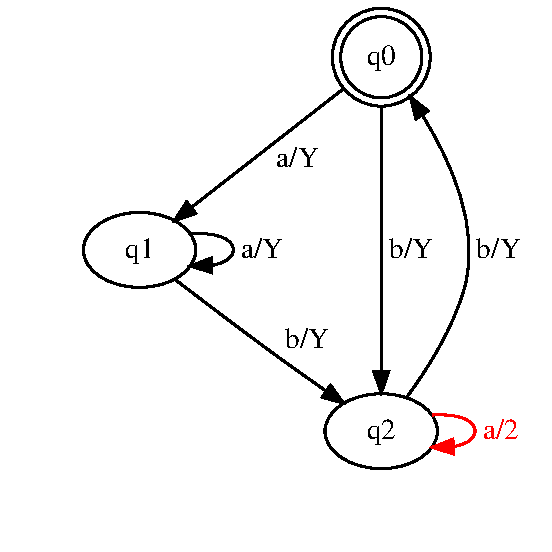
\includegraphics[width=\textwidth]{images/fsm-example01_abs}}%
\only<2->{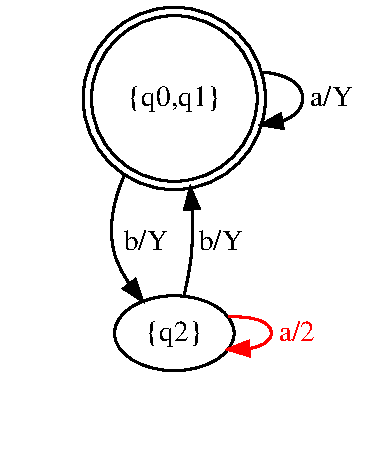
\includegraphics[width=0.8\textwidth]{images/fsm-example01_abs_min}}%
\end{column}%
\end{columns}
\end{frame}

\begin{frame}
\frametitle{Safety-H Methode}
$(\alpha, \beta)$-Liste stammt aus den gleichen Mengen wie bei der $H$-Methode
\begin{itemize}
    \item $A=V\times V$
    \item $B=V\times (V.\bigcup\limits_{i=1}^{m-n+1}.\Sigma_I^i)$
    \item $C=\{(\alpha,\beta)|\alpha,\beta\in V.\bigcup\limits_{i=1}^{m-n+1}.\Sigma_I^i, \alpha \in \text{Pref}(\beta)\}$
  \end{itemize}

\begin{columns}[T] % align columns
\begin{column}{.50\textwidth}
\pause
\begin{itemize}
  \item<2-> $(\alpha, \beta) \in A, \delta(q_0,\alpha) \not \sim \delta(q_0, \beta)$
  \item<3-> $(\alpha, \beta) \in B, \delta(q_0,\alpha) \not \sim_s \delta(q_0, \beta)$
  \item<3-> $(\alpha, \beta) \in C, \delta(q_0,\alpha) \not \sim_s \delta(q_0, \beta)$
\end{itemize}
  \end{column}%
  \begin{column}{.60\textwidth}

  \begin{itemize}
  \item[]<2-> \textcolor{blue}{\underline{\textcolor{black}{Wie in $H$-Methode}}}
  \item[]<3-> \textcolor{red}{\underline{\textcolor{black}{Weniger Zustände unterscheidbar}}}
\end{itemize}
  \end{column}
\end{columns}
\end{frame}

\begin{frame}
\frametitle{Safety-H Methode}
\begin{itemize}
  \item Verallgemeinerung der $H$-Methode
  \item Je weniger Zustände die Abstraktionsmaschine hat, desto weniger Testfälle werden erzeugt
\end{itemize}
\end{frame}

\begin{frame}
\frametitle{Algorithmus für safety-H Methode (1)}
Input: vollständige, minimale Referenz-DFSM $Ref_min$ und dazugehörige minimierte Abstraktions-DFSM\\
Output: safety-Testsuite
\begin{enumerate}
  \item Füge $V.\bigcup\limits_{i=1}^{m-n+1}.\Sigma_I^i$ der Testsuite hinzu
  \item Generiere Menge $A$, $B$ und $C$ aus der vollständigen, minimalen Referenz-DFSM
  \item Generiere $(\alpha, \beta)$-Liste aus $A$
  \item Iteriere über Liste:
  \begin{itemize}
    \item Berechne Zustand $q = \delta(q_0,\alpha)$ und $q'=\delta(q_0,\beta)$ in der \textbf{Referenzmaschine}
    \item Falls $q = q'$: Wähle $\omega$ und füge $\alpha.\omega$ sowie $\beta.\omega$ der Testsuite hinzu
  \end{itemize}
\end{enumerate}
\end{frame}

\begin{frame}
\frametitle{Algorithmus für safety-H Methode (1)}
\begin{enumerate}
  \setcounter{enumi}{4}
  \item Generiere neue $(\alpha, \beta)$-Liste aus $B$ und $C$
  \item Iteriere über Liste:
  \begin{itemize}
    \item Berechne Zustand $q = \delta(q_0,\alpha)$ und $q'=\delta(q_0,\beta)$ in der \textbf{Abstraktionsmaschine}
    \item Falls $q = q'$: Wähle $\omega$ und füge $\alpha.\omega$ sowie $\beta.\omega$ der Testsuite hinzu
  \end{itemize}
\end{enumerate}
\end{frame}

\begin{frame}
\frametitle{Algorithmus für safety-H Methode (2)}
Input: vollständige, minimale Referenz-DFSM $Ref_{min}$ und dazugehörige minimierte Abstraktions-DFSM\\
Output: safety-Testsuite
\begin{enumerate}
  \item Iteriere über $(\alpha,\beta)$-Liste und erzeuge $TS_1$ wie in (1)
  \item Iteriere über $(\alpha,\beta)$-Liste rückwärts (zufällige Reihenfolge) und erzeuge $TS_2$
  \item Starte ALgorithmus neu mit $TS_1 \cap TS_2 (\cap TS_i)$
\end{enumerate}
\end{frame}

\begin{frame}
\frametitle{Minimale Testsuite?}
\begin{itemize}
  \item Minimale Testsuite zu finden ist ein NP-vollständiges Problem
  \item Reihenfolge der Bearbeitung beeinflusst das Ergebnis
  \item Wegen veränderter Reihenfolge kann $TS_s$ größer werden als $TS$
\end{itemize}
\end{frame}

\begin{frame}
\frametitle{Algorithmus für safety-H Methode (3)}
Input: vollständige, minimale Referenz-DFSM $Ref_{min}$ und dazugehörige minimierte Abstraktions-DFSM\\
Output: safety-Testsuite
\begin{enumerate}
  \item Führe die $H$-Methode durch und merke, welcher Test durch welches $(\alpha,\beta)$-Paar zustandegekommen ist, und ob dieser wegen $A$ hinzugefügt wurde.
  \item Iteriere über Tests
  \begin{enumerate}
    \item Iteriere über alle $(\alpha,\beta)$-Paar für diesen Test\\
    \begin{itemize}
      \item[] Falls $(\alpha,\beta)$-Paar wegen A erzeugt wurde: Nächstes Paar
      \item[] Falls für alle gilt $\delta(q_0,\alpha) = \delta(q_0,\beta)$ \textbf{in der Abstraktionsmaschine}
      \item[] $\Rightarrow$ Test kann entfernt werden

    \end{itemize}
  \end{enumerate}
\end{enumerate}
\end{frame}

\begin{frame}
\frametitle{Vergleich}
\begin{table}[]
\centering
\begin{tabular}{|l|l|l|l|}
\hline
m=n                    & H Methode & s-H Methode & Verbesserung \\\hline
FSBRTS                 & 511       & 337         & 34 \%        \\
Synthetic              & 61        & 31          & 49 \%        \\
Garage Door Controller & 13        & 13          & 0 \%         \\
\hline
\end{tabular}
\end{table}
\end{frame}

\begin{frame}
\frametitle{Beispiel: Garage Door Controller}
Fernbedienung mit einer Taste steuert Garagentür
Garagentür kann:
\begin{itemize}
	\item herunterfahren
	\item hochfahren
	\item stoppen
	\item Richtung wechseln
	\item Lichtschranke aktivieren und stoppen
\end{itemize}

\end{frame}
\begin{frame}
\frametitle{Beispiel: Garage Door Controller}
\centering
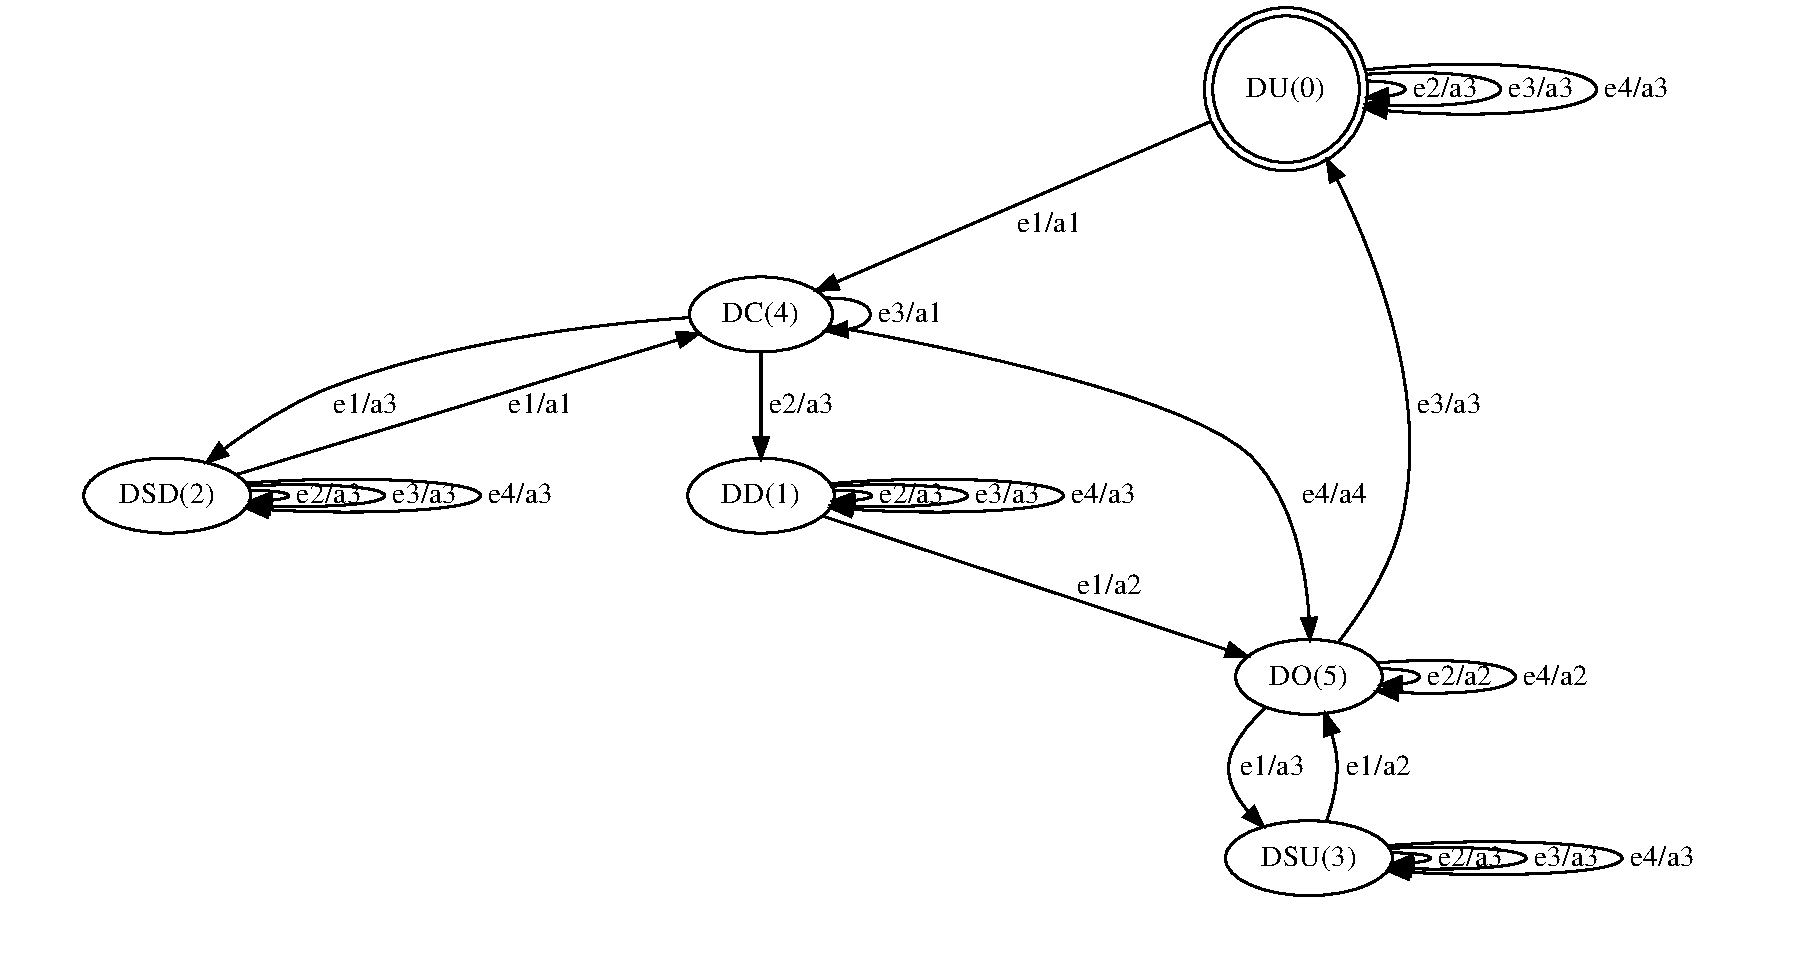
\includegraphics[width=1.15\textwidth]{images/gdc}

\end{frame}


\begin{frame}
\frametitle{Beispiel: Garage Door Controller}
\begin{columns}[T] % align columns
\begin{column}{.55\textwidth}

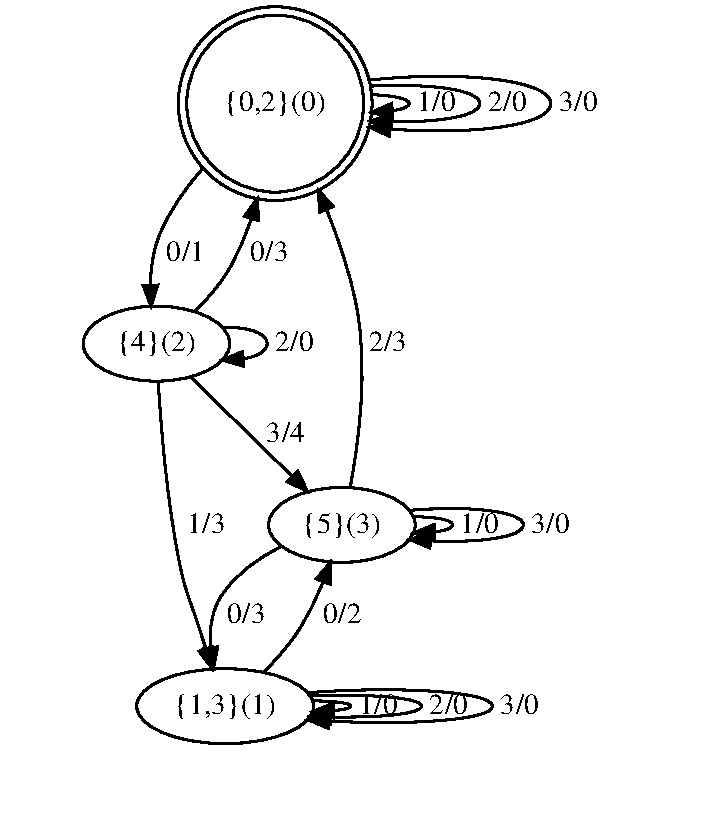
\includegraphics[width=\textwidth]{images/gdc_min}
\end{column}%
\hfill%
\begin{column}{.55\textwidth}
Eingabe:
\begin{itemize}
  \item e1: Fernbedienung gedrückt
  \item e2: Sensor "Tür ist unten"
  \item e3: Sensor "Tür ist oben"
  \item e4: Sensor "Lichtschrank aktiviert"
\end{itemize}
Ausgabe:
\begin{itemize}
  \item a1: "Tür fährt herunter"
  \item a2: "Tür fährt hoch"
  \item a3: "Stop"
  \item a4: "Richtungswechsel unten $\rightarrow$ oben"
\end{itemize}
\end{column}%
\end{columns}
\end{frame}

\begin{frame}
\frametitle{Beispiel: Garage Door Controller}
\begin{columns}[T] % align columns
\begin{column}{.55\textwidth}

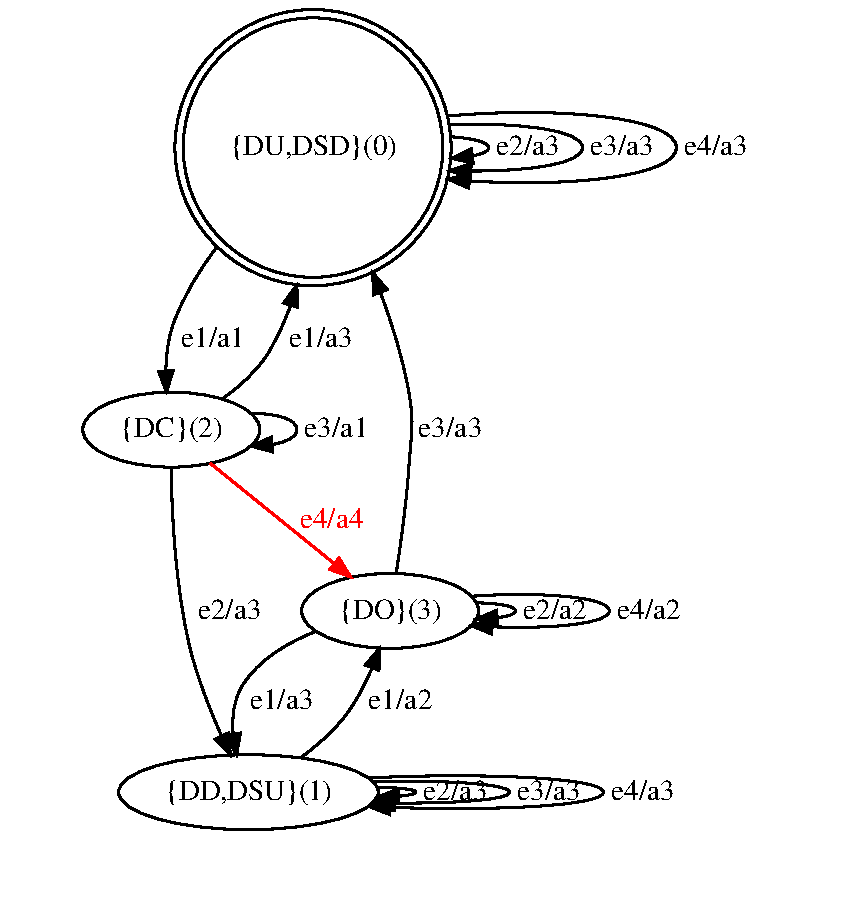
\includegraphics[width=\textwidth]{images/gdc_min_colored}
\end{column}%
\hfill%
\begin{column}{.55\textwidth}
Eingabe:
\begin{itemize}
  \item e1: Fernbedienung gedrückt
  \item e2: Sensor "Tür ist unten"
  \item e3: Sensor "Tür ist oben"
  \item e4: Sensor "Lichtschrank aktiviert"
\end{itemize}
Ausgabe:
\begin{itemize}
  \item a1: "Tür fährt herunter"
  \item a2: "Tür fährt hoch"
  \item a3: "Stop"
  \item a4: "Richtungswechsel unten $\rightarrow$ oben"
\end{itemize}
Sicherheitskritisch ist nur \textcolor{red}{a4}.
\end{column}%
\end{columns}
\end{frame}

\begin{frame}
\frametitle{Beispiel: Garage Door Controller}
\begin{columns}[T] % align columns
\begin{column}{.53\textwidth}

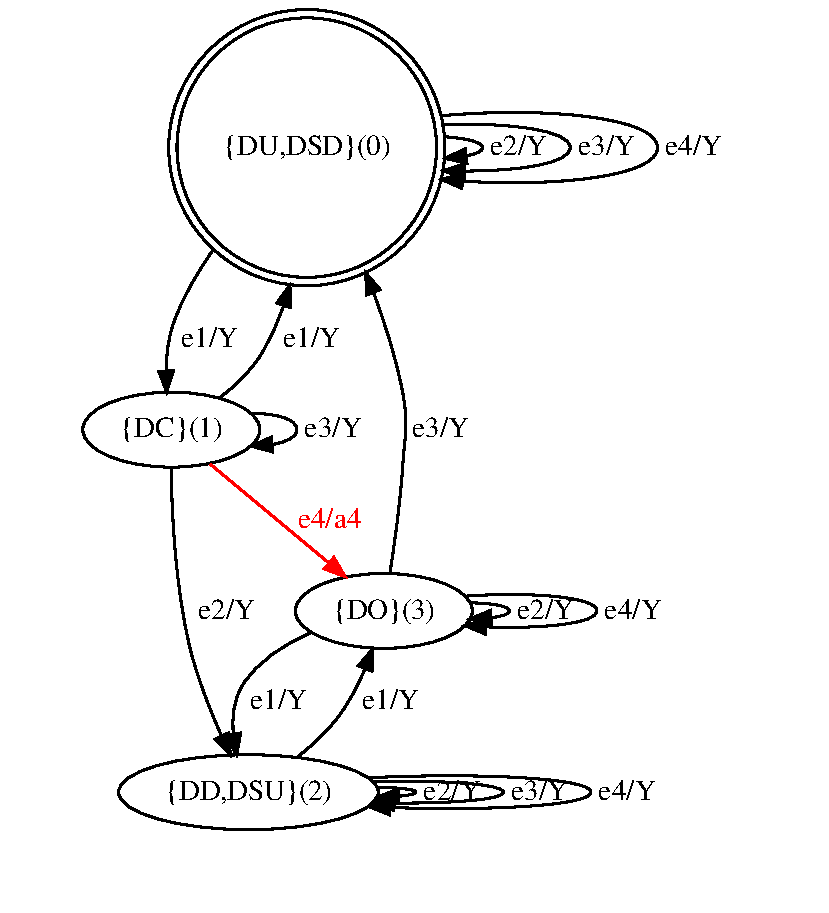
\includegraphics[width=\textwidth]{images/gdc_abs_min_colored}
\end{column}%
\hfill%
\begin{column}{.55\textwidth}
Eingabe:
\begin{itemize}
  \item e1: Fernbedienung gedrückt
  \item e2: Sensor "Tür ist unten"
  \item e3: Sensor "Tür ist oben"
  \item e4: Sensor "Lichtschrank aktiviert"
\end{itemize}
Ausgabe:
\begin{itemize}
  \item a4: "Richtungswechsel unten $\rightarrow$ oben"
  \item Y: Sonstige
\end{itemize}
Sicherheitskritisch ist nur \textcolor{red}{a4}.
\end{column}%
\end{columns}
\end{frame}

\section{Ausblick}
\begin{frame}
\frametitle{Ausblick}
  \begin{itemize}
    \item Implementationen verifizieren
    \item Random-Generator für minimierbare DFSMs
    \item Ausführliche Experimente über Reduktion von $TS_H$ zu $TS_{sH}$
  \end{itemize}
\end{frame}


\end{document}


